% !TEX root = ../thesis.tex

\documentclass[thesis.tex]{subfiles}

% Johdanto selvittaa samat asiat kuin tiivistelma, mutta laveammin. Johdannossa kerrotaan yleensa seuraavat asiat
% \item[--]Tutkimuksen taustaa ja tutkimusaiheen yleisluonteinen esittely
% \item[--]Tutkimuksen tavoitteet
% \item[--]Paakysymys ja osaongelmat
% \item[--]Tutkimuksen rajaus ja keskeiset kasitteet
% Aiheen rajaus johdantoon.

\begin{document}

\chapter{Introduction}
\label{chapter:intro}

Numeric Identifier/ One dimension-Bar Code
QR code and other two dimensional bar codes
3. Physical Fingerprint Technology on visible spectrum: holograms, paper, inks, security threads and regardless it is overt or covert.
NFC Radio Frequency Identifier (RFID)

Driving smartphones forward as an authentication device has not only been their automation, but also their convenience. Concurrently, anti-counterfeit solutions offering high levels of security are also often costly to implement, making them difficult to afford. It is therefore highly desirable to consider technologies that are both secure and cost-effective, and do not require special readers to be detected.

Most importantly, unlike special reading devices, smartphones provide true portability and rapid deployment, making it possible to develop an authentication application that will work in different environments and be distributed in multiple markets, without adapting the hardware or the source code.

% http://ipimediaworld.com/wp-content/uploads/2013/10/Turning-your-smartphone.pdf

vaarentajat pyrkivat selvittamaan tekniikan periaatteen nopeasti, joten turvallisuussovelluksissa kaytettavia merkintoja on oltava riittavan monimutkaisia ja niita on voitava muunnella helposti. luminoforien luminesenssiominaisuudet muuttuvat yhdisteen rakenteen muuttuessa. Erilaisten rakenteiden suunnitelmallinen synteesi onkin tarkeaa, mikali tekniikkaa halutaan kehittaa eteenpain. Luminoforien viritys- ja emissioaallonpituuksien tulisi soveltua myos kaytetyn laitteiston vaatimuksiin.


on the product surfaces and on their packages
Important application fields are e.g. packages of medicines and expensive products and their packages. Developed markings are typically not visible for the bare eyes.

- Tools for identifying counterfeit goods
- OECD has estimated the value of internatioanlly traded counterfeit products in 2015 would be 770-990 billion US
- low cost marking technology for production authentication/track-and-trace purposes
- portable low-cost, handheld reading instrument
- printable
- stakeholders: brand owners, distributions, packaging industry, authorities

% Product authentication, or brand protection, ...
% This thesis explores an alternative, competing technology.

%Moreover, usability is improved as the application can function offline without the overhead of network latency. Hosting fingerprint data on the user's device might however have security implications: can the data be safely/efficiently encrypted on the user's device? The product authentication ecosystem \ref{fig:landscape}.
http://www.iccwbo.org/Advocacy-Codes-and-Rules/BASCAP/BASCAP-Research/Economic-impact/Global-Impacts-Study/
\begin{figure}[h!]
\centering 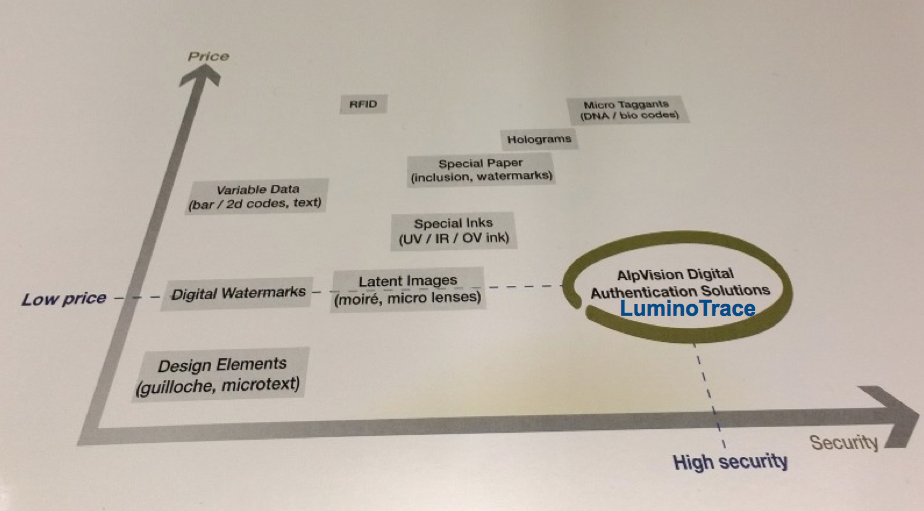
\includegraphics[width=\linewidth]{images/landscape}
\caption{Product authentication landscape \label{fig:landscape}}
\end{figure}

\section{Research Questions}
\label{chapter:research-questions}

This thesis aims to answer the following questions:

\begin{itemize}
  \item \label{RQ1} \textbf{RQ1}: How can photoluminescence and smartphones be integrated for product authentication purposes?
  \item \label{RQ2} \textbf{RQ2}: Which factors affect the analysis of photoluminescent material (luminophores) in the context of smartphones?
  \item \label{RQ3} \textbf{RQ3}: Does modern smartphone technology provide the means for photoluminescence based product authentication in practice?
\end{itemize}


\end{document}